\documentclass{beamer}
\usepackage{german}
\usepackage{graphicx}
\usepackage{listings}

% https://github.com/FuzzyWuzzie/Beamer-Theme-Execushares
\usetheme{Execushares}

\begin{document}

\title{Vert.x Clustering}
\author{Felix Hamann}
\date{23. Juni 2016}


\begin{frame}
\titlepage
\end{frame}


\begin{frame}
  \frametitle{Was ist Clustering?}

  \begin{itemize}
    \item Ein Zusammenschluss homogener Computer
    \item Jeder Computer erfüllt die gleiche Aufgabe
    \item In der Regel per lokalem Netzwerk verbunden
    \item Verhält sich wie ein großer Rechner
  \end{itemize}

\end{frame}


\begin{frame}
  \frametitle{Warum clustern?}

  \begin{itemize}
    \item Ausfallsicherheit erhöhen
    \item Für Hochverfügbarkeitssysteme
    \item Um Supercomputer zu bauen
    \item Variabel auf Lastschwankungen reagieren (IaaS/PaaS)
    \item Kann kosteneffizient sein
  \end{itemize}

\end{frame}


\begin{frame}
  \frametitle{Vert.x Architektur}
  \vspace{1cm}

  \begin{center}
    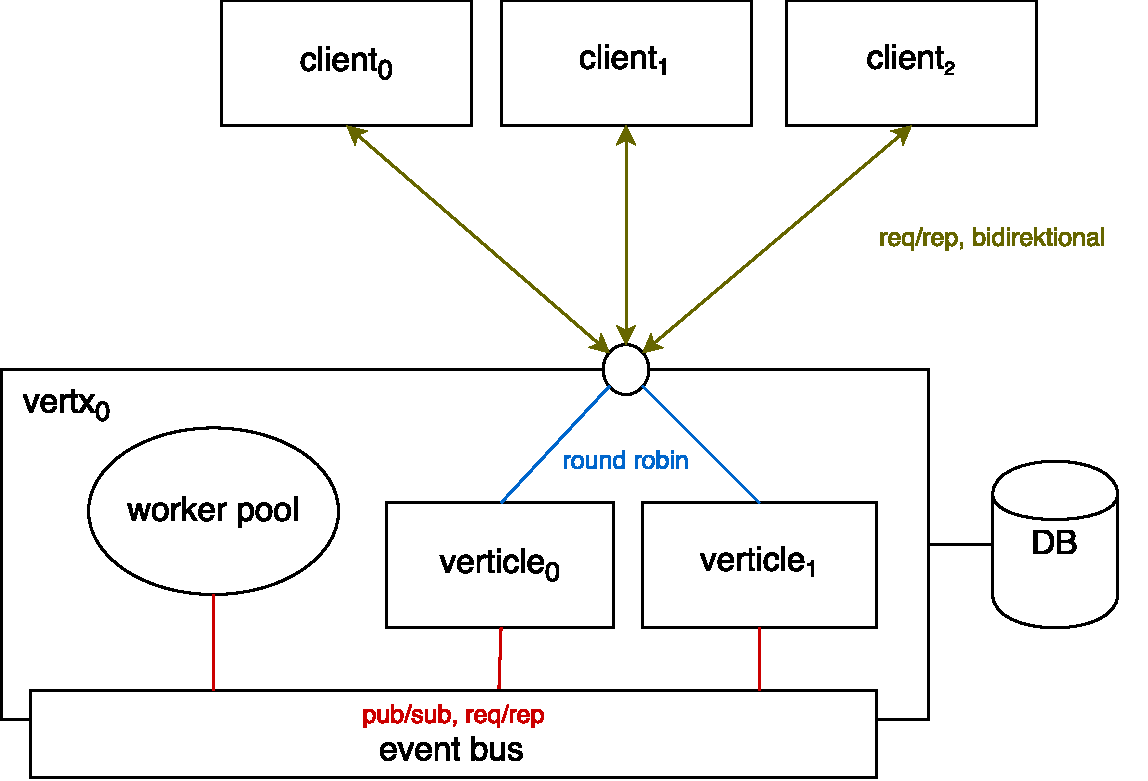
\includegraphics[height=5cm]{src/single_deployment.pdf}
  \end{center}
\end{frame}


\begin{frame}
  \frametitle{Clustering bei Vert.x}
  \vspace{1cm}

  \begin{enumerate}
    \item Optionen setzen
    \item Vert.x asynchron starten
    \item Profit
  \end{enumerate}

  \line(1,0){250}

  \lstinputlisting[language=Java]{src/vertx_async.java}
\end{frame}



\begin{frame}
  \frametitle{Vert.x Cluster Beispiel-Architektur}
  \vspace{1cm}

  \begin{center}
    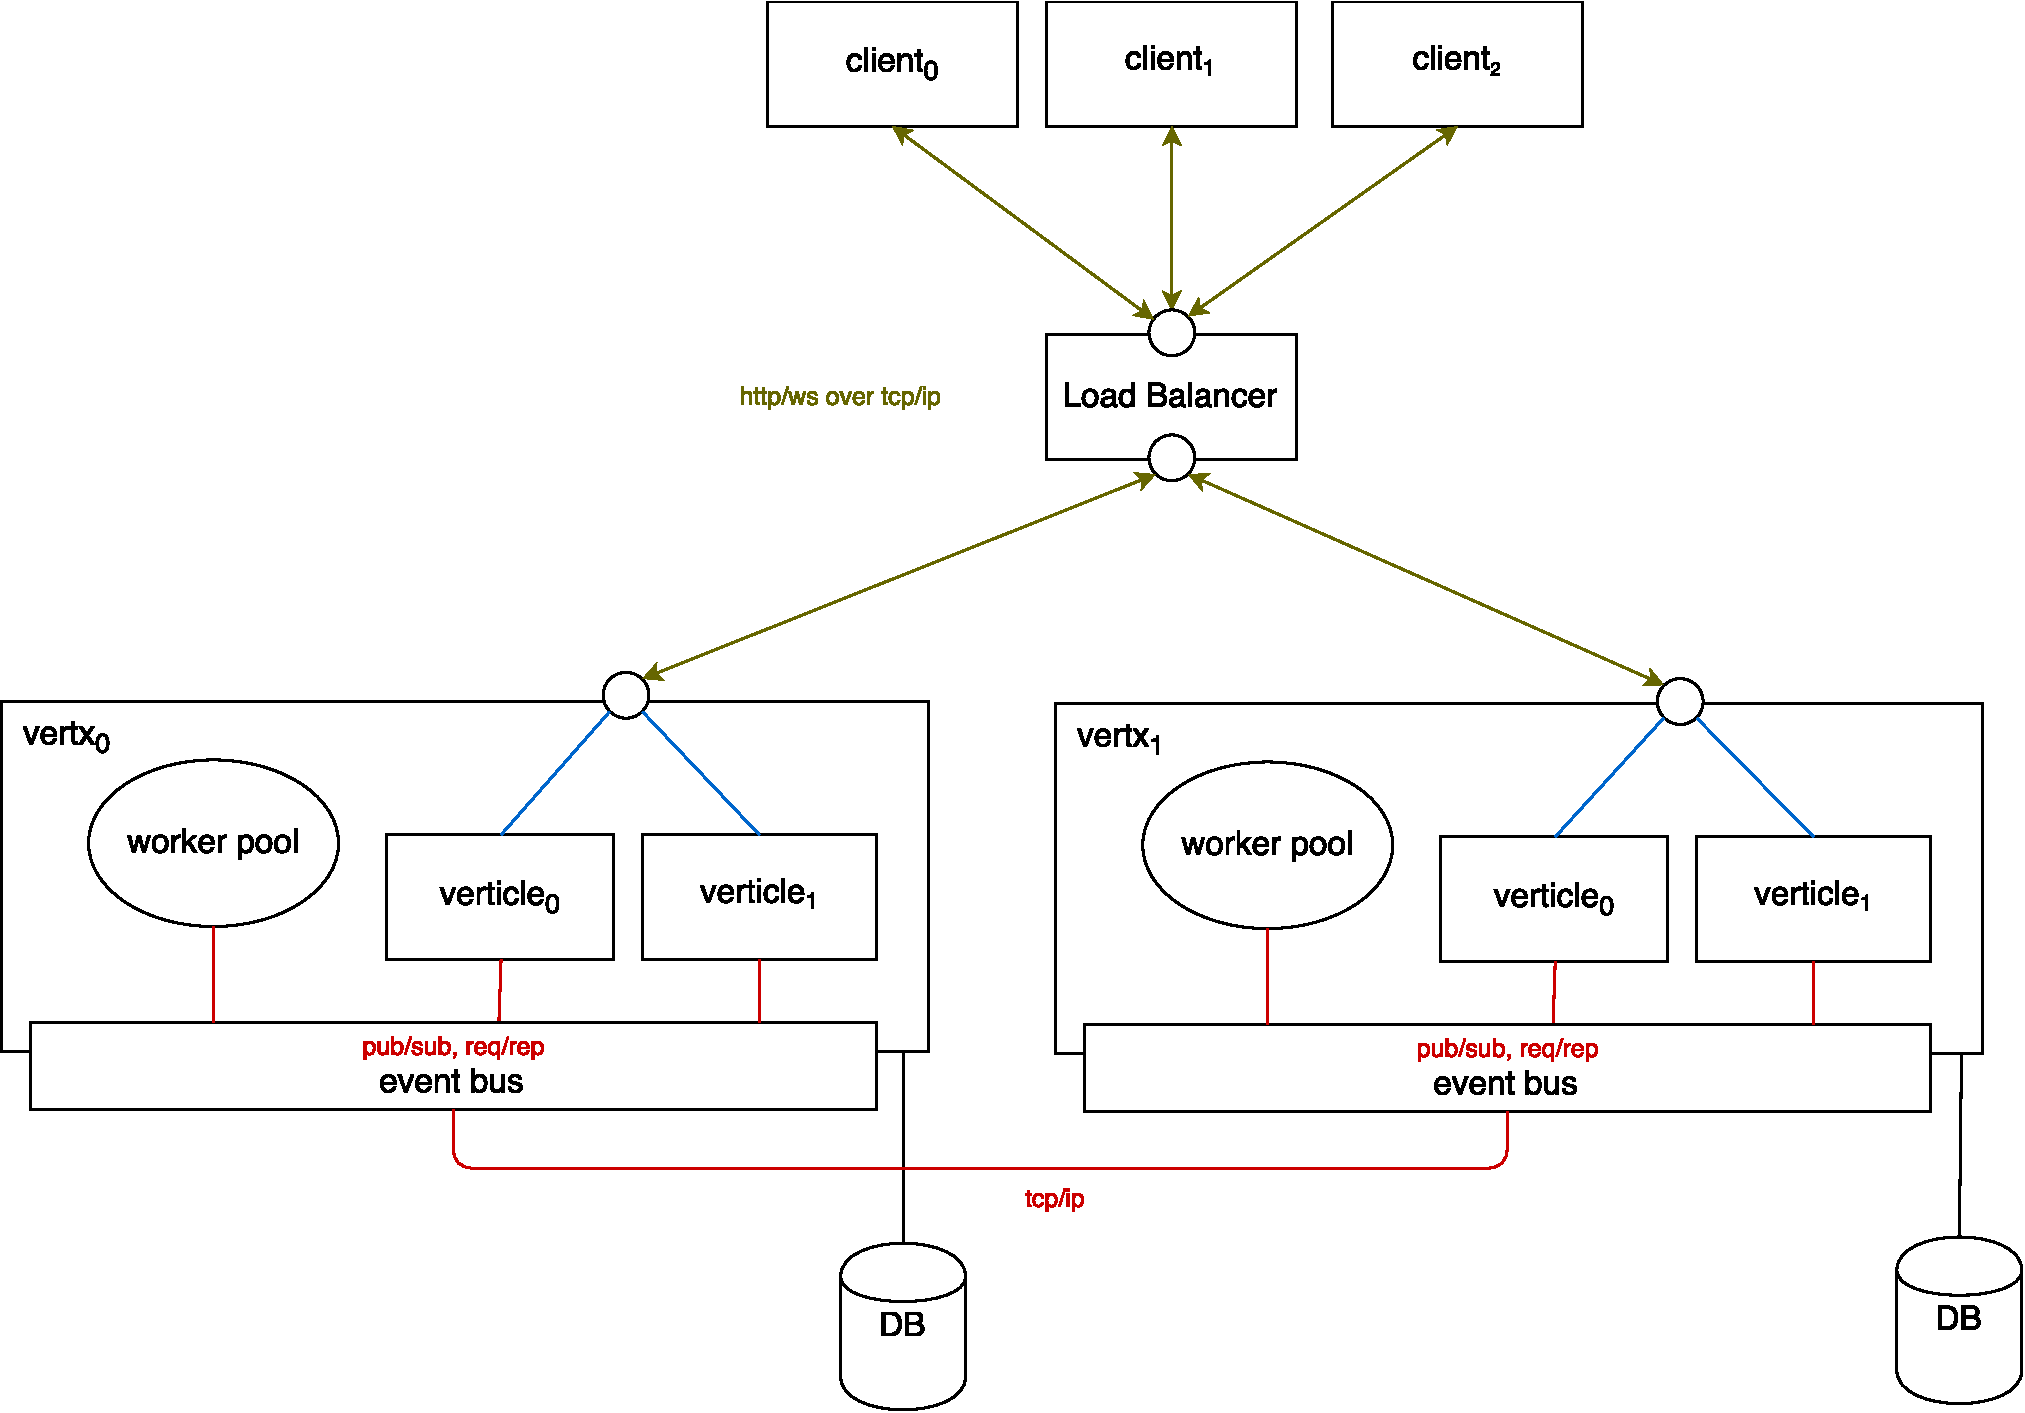
\includegraphics[height=7cm]{src/cluster_deployment.pdf}
  \end{center}
\end{frame}

\begin{frame}
  \frametitle{Shared Data}
  \vspace{1cm}

  \begin{enumerate}
    \item LocalMap pro Instanz sichtbar
    \item AsyncMap pro Cluster
    \item Atomare Counter
    \item Verteilte Locks
  \end{enumerate}
  \vspace{.1cm}

  \begin{center}
    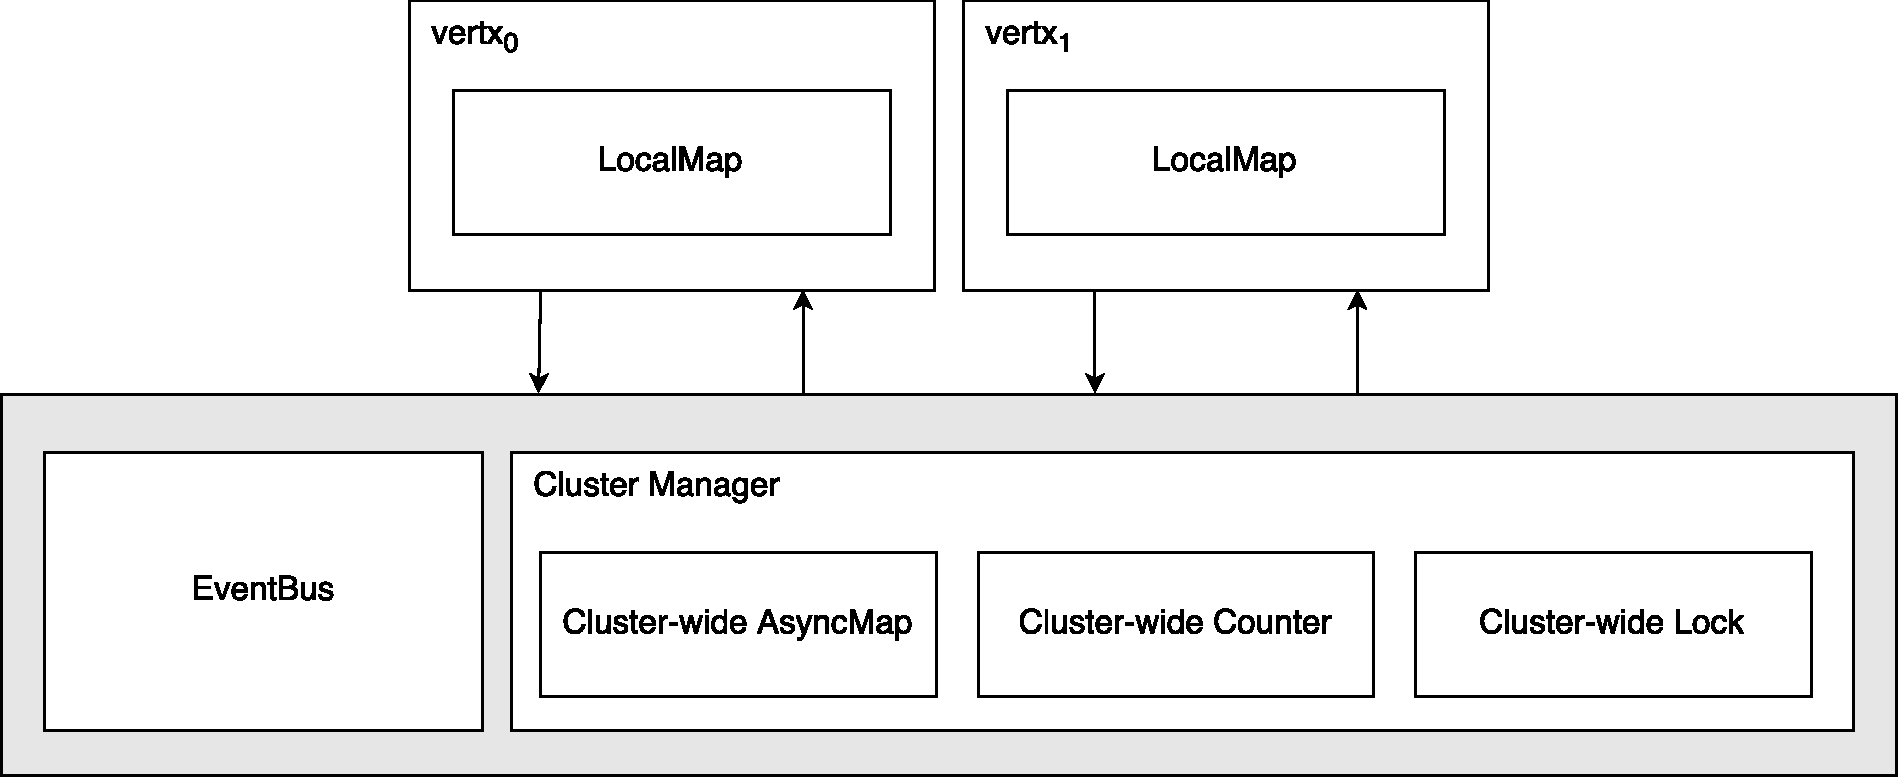
\includegraphics[height=4cm]{src/shared_data.pdf}
  \end{center}

\end{frame}


\begin{frame}
  \frametitle{Local Shared Map}

  Synchrones Interface zum Austausch von unveränderlichen Daten
  zwischen verschiedenen Verticle-Instanzen

  \vspace{.3cm}
  \line(1,0){250}
  \vspace{.3cm}

  \lstinputlisting[language=Java,basicstyle=\scriptsize]{src/localmap.java}
\end{frame}


\begin{frame}
  \frametitle{Cluster Wide Map}
  \vspace{.5cm}

  Asynchrones Interface um Daten quer über den gesamten Cluster auszutauschen.
  Kann zB. verwendet werden um Nutzersessions zu verwalten.

  \vspace{.3cm}
  \line(1,0){250}
  \vspace{.3cm}

  \lstinputlisting[language=Java,basicstyle=\scriptsize]{src/asyncmap.java}
\end{frame}


\begin{frame}
  \frametitle{Lock und Counter}
  \vspace{1cm}

  \lstinputlisting[language=Java,basicstyle=\scriptsize]{src/lock_counter.java}
\end{frame}


\begin{frame}
  \frametitle{Demo}
  \vspace{1cm}

  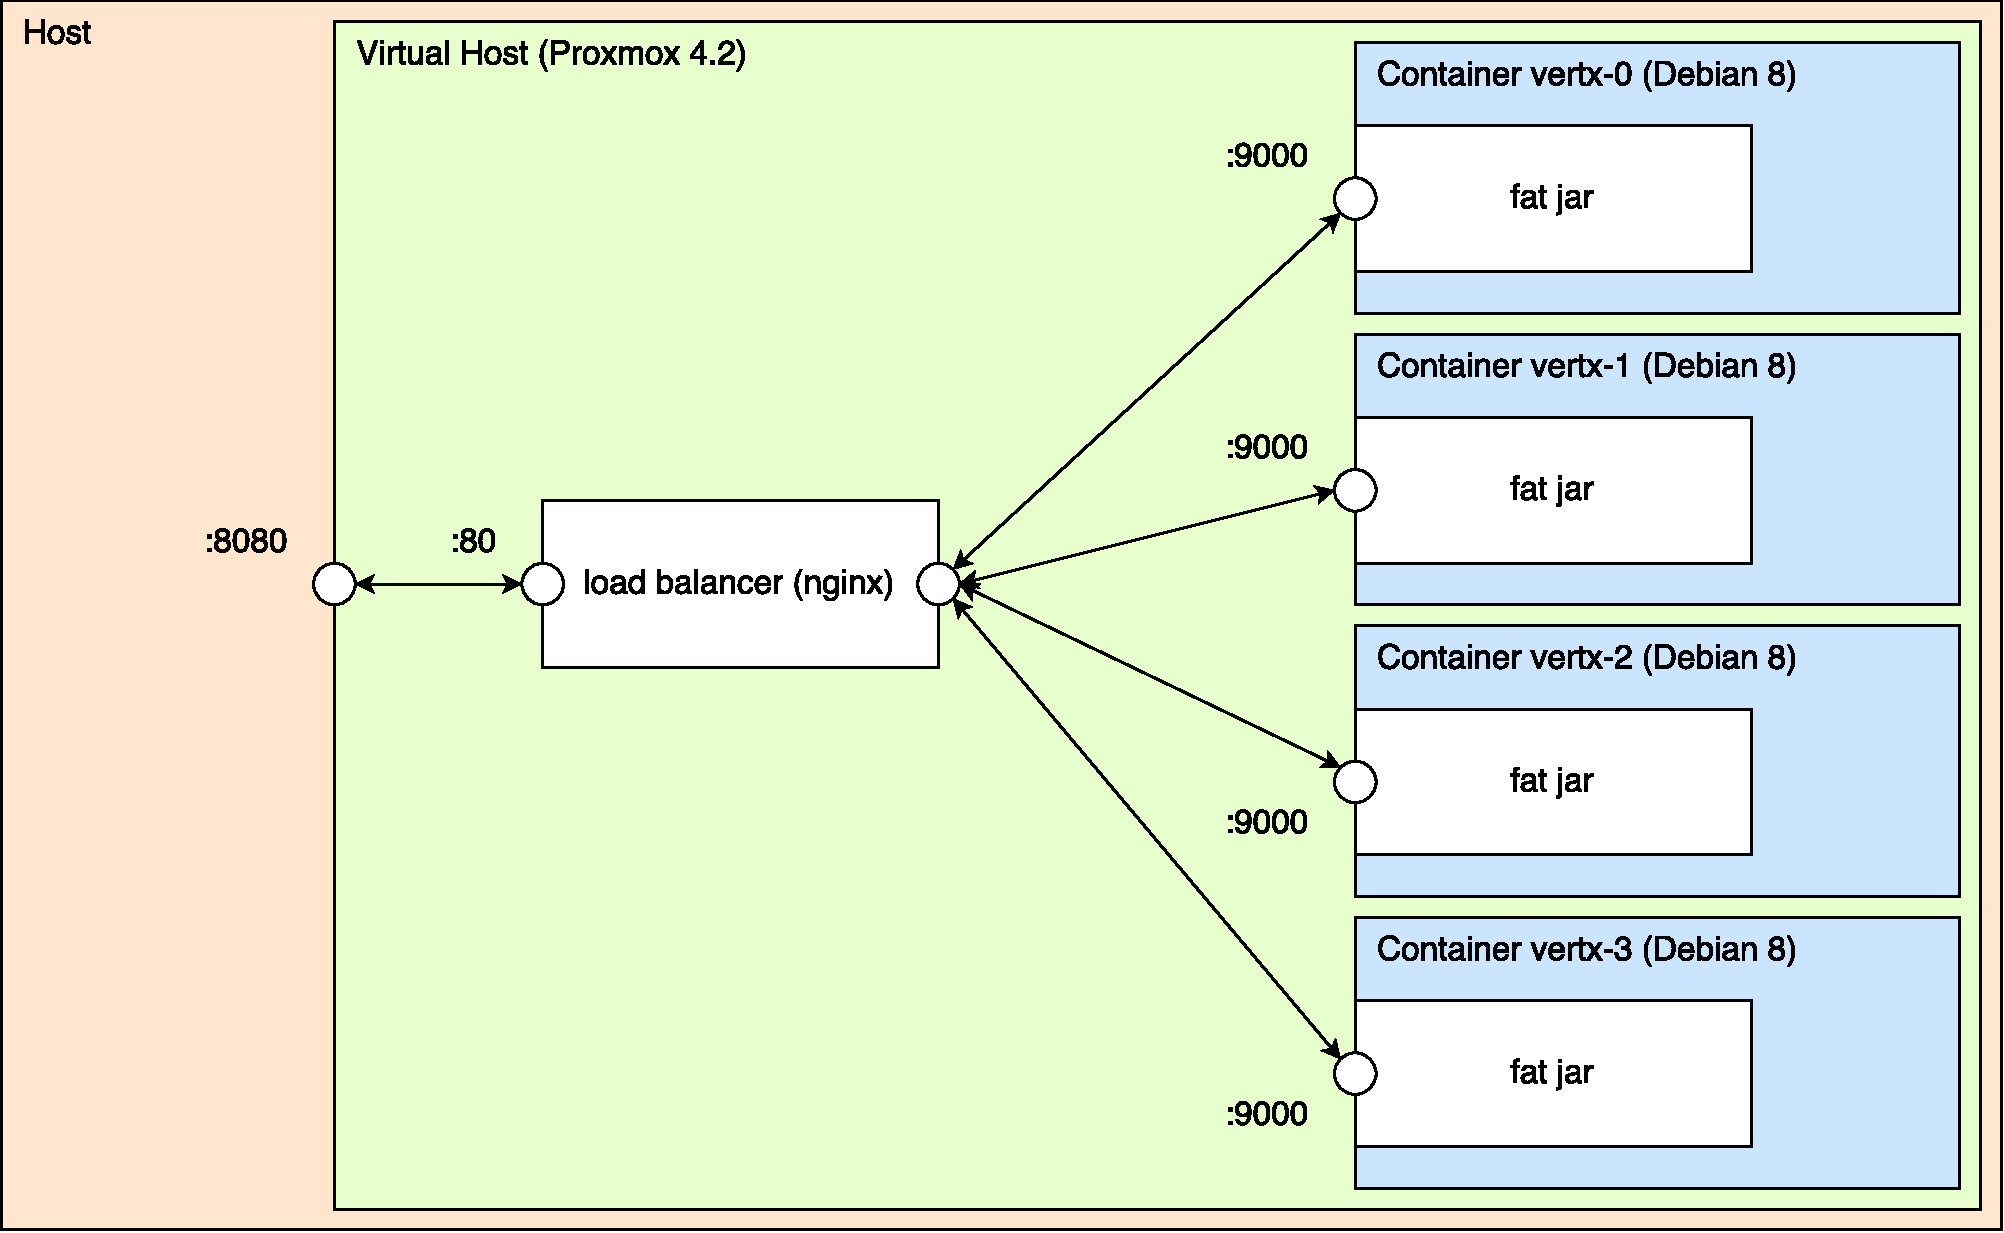
\includegraphics[height=6cm]{src/demo.pdf}
\end{frame}


\begin{frame}
  \frametitle{Fazit}

  \begin{itemize}
    \item Ob Clustering nötig ist, ist abhängig von der individuellen Architektur (SOA vielleicht, Microservices nein)

    \item Notwendig für Hochverfügbarkeit (wenn man das denn braucht)

    \item Einfaches Mittel zum ad-hoc skalieren, aber der Preis ist die Komplexität eines verteilten Systems

    \item Bei I/O lastigen Systemen ist Vert.x wohl selten der Flaschenhals

    \item Allgemein: Je weniger State im Service, umso weniger Kopfschmerz
  \end{itemize}
\end{frame}


\end{document}